\documentclass[male, authorStatement, indexNumber, fileVersion, keywords, thanks]{lib/uekthesis}
\usepackage{lib/uekthesis}


%##############################################################################
% Zmienne Globalne !!! - ważne by kodowanie UTF-8 było wstawione przed nimi
%
% To zmiennne do modyfikacji przez użytkownika
%
\globalFullAuthor{Jan Kowalski}                     % Pełna nazwa autora pracy
\globalShortAuthor{J.\ Kowalski}                     % Autor - zwięzła forma wydruku
\globalFullTitle{Przygotowanie pracy dyplomowej \\[2mm] wraz z systemem LaTeX}  % Pełny tytuł pracy
\globalShortTitle{Praca dyplomowa w systemie LaTeX}       % Krótki, zwięzły tytuł pracy
\globalFullUniversity{Uniwersytet Ekonomiczny w Krakowie} % Pełna nazwa uniwersytetu
\globalShortUniversity{UEK}                           % Skrócona nazwa uniwersytetu
\globalDepartment{Wydział Zarządzania}                % Wydział
\globalDegreeprogramme{Informatyka Stosowana}         % Kierunek studiów
\globalThesisType{Praca dyplomowa}                    % Typ pracy dyplomowej
\globalUnderTheSupervisonOf{Pod kierunkiem}
\globalSupervisor{prof. n. dr hab. Jana Iksińskiego}  % Promotor
\globalAcknowledgements{Dla moich rodziców oraz najbliższych przyjaciół za niezłomną wiarę w~moje zwycięstwo.}   % Podziękowania
\globalFileVersion{0.1.0}   % wersja pliku
\globalIndexNumber{123456}  % wersja pliku
\globalCity{Kraków}         % miasto
\globalYear{2015}           % rok powstania pracy
\globalKeywords{nauka, komputery, praca dyplomowa, latex, uczelnia, student} % słowa kluczowe dla pracy

%##############################################################################
% Dołączenie pliku bibliografii zgodnej z Biblatex
\addbibresource{bibliography.bib}

%##############################################################################
% dodatkowe pakiety
\usepackage{chemfig} % wzory chemiczne

% Lista słów (dzielenia je, lub nie)
\hyphenation{LaTeX latex LaTeXu}

%##############################################################################
% Koniec preambuły i rozpoczęcie treści właściwej dokumentu
\begin{document}
\nocite{*}

\titlepages
\tableofcontents
\clearpage

% Tu umieszczamy rozdziały w porządanej kolejności 
\chapter*{Wstęp}
\label{chap:wstep}
\addcontentsline{toc}{chapter}{Wstęp}
\addtocounter{chapter}{0}
\sectionmark{Wstęp} % changes the head for the current page

Oto kilka słów wstępu dla początkowego rozdziału publikacji rozpoczynającego dywagację autora na temat jego pracy. 

Jak widać rozdział ten nie zawiera numeracji, co zwykle jest bardzo porządaną cechą dla rozdziału wprowadzającego czytelnika w całość dokumentu. \\
Nastomiast jak zostało to dokonane można bez trudu podejrzeć w pierwszych 5 linijkach kodów źródłowych pliku \path{chap_0_intro.tex} zamieszczonego na stronie \url{https://github.com/egel/latex-thesis-example}.

Zapraszam serdecznie do przejrzenia i wypróbowania niniejszego repozytorium.




\chapter{Teoretyczne podwaliny}
\label{chap:teoretyczne_podwaliny}

Treść dla rozdziału pierwszego zwykle zawiera w sobie teoretyczne podwaliny pod dalszą część Twojej pracy dyplomowej (czy to licencjackiej, magisterskiej lub nawet doktorskiej). 

Jak również zapewne zauważyłeś drogi Czytelniku, rozdział ten posiada już normalną numerację, tak jak to powinno wyglądać w wydruku dla pracy końcowej (patrz spis treści).

\begin{table}[!h]
    \centering
    \begin{tabular}{|c|c|}
    \hline
    \textbf{Kolumna 1} & \textbf{Kolumna 2} \\ \hline \hline
    wiersz1-kolumna1 & wiersz1-kolumna2 \\ \hline
    wiersz2-kolumna1 & wiersz2-kolumna2 \\ \hline
    \end{tabular}
\caption{Prosta tabelka dla przykładu}
\label{tab:tab:prosta-tabela-przyklad-A}
\end{table}


\section{Przykładowy podrozdział 1-go rzędu}
Jak widać można zagnieżdżać treści w wygodne sekcje (ang. \textit{sections}) tak jak również w~dowolnym momencie umieszczać rysunki lub fotografie --- tak jak to widać na rysunku~\ref{fig:word-vs-latex}.

\begin{figure}[!ht]
\centering
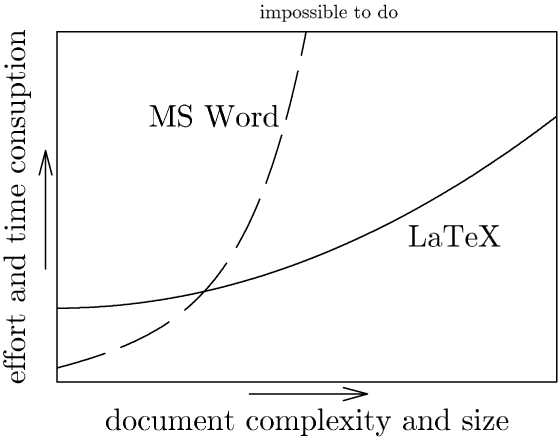
\includegraphics[width=100mm]{images/word-vs-latex.png}
\captionsource{Trudnośc pisania dokumentów w stosunku do ich objętości}{\url{http://www.pinteric.com/miktex.html}}
\label{fig:word-vs-latex}
\end{figure}

Czasem zdaży się również tak, że przeniesie zdjęcie na kolejną stronę, jednak w~pewnych okolicznościach to celowy zabieg który wykonuje za nas kompilator LaTeXa --- Super! :) \\
Wtedy można bez kołototu odwołać się do konkretnego zdjęcia, tabeli, kodu źródłowego, przypisu bibliograficznego, ect. poprzez referecję (komendę \texttt{\textbackslash{}ref\{?\}} i podanie zamiast znaku zapytania odwołania, czyli tzw. \texttt{label}-ki). Całość opisaną powyżej mozna odnaleźć w kodzie źródłowym do niniejszego rozdziału. Tak, to na prawdę jest, aż takie proste :)

\subsection{Podrozdział 2-go rzędu}
\label{subsec:podrozdzial-2-rzedu}

A tu przykład kolejnego zagnieżdzenia. Zwylke wystarczają 2 w 3 stopniowej skali: rozdział, pod-rozdział, pod-pod-rozdział. Można równie łatwo się do nich odwoływać, niezależnie od kolejności --- czy to w postaci napisu tj. \nameref{chap:praktyczne-zastosowanie}, czy też w postaci liczby określającej go, tj.~\ref{chap:praktyczne-zastosowanie}.
\chapter{Praktyczne zastosowanie}
\label{chap:praktyczne-zastosowanie}

Treść dla niniejszego rozdziału to zwykle praktyczne zastosowanie omawianego zagadnienia. Poprzez analizę rozdziału \nameref{chap:teoretyczne_podwaliny}, a~także jego wykorzystanie w~praktyce, dyplomanta stara się nakreślić całość rozdziału praktycznego.

\section{Tworzenie obiektów LaTeXa}
\label{sec:tworzenie-obiektow-latexa}
Oprócz tego że mozemy ładnie dzielić treści, umieszczać zdjęcia, tabele, kody źródłowe, odwoływac się do przypisów bibliograficzych, możemy także\footnote{Tworzyć przypisy dolne w miejscu w którym rzeczywiście powinnu się znaleść, a LaTeX przygotuje i sformatuje je za nas!}:

\note{\textbf{Pamietaj!} LaTeX jest bardzo skrupulatny, tak więc istnieje dla niego widoczna różnica pomiędzy \textbf{przypisem dolnym} (który zaobserowowałeś powyżej, \texttt{\textbackslash{}footnote\{\}}), a \textbf{odwołaniem do bibliografi umieszczonym w przypisie dolnym} (\texttt{\textbackslash{}footcite\{\}}). \\
Dla więkości osób piszących na codzień teksty w Wordzie nie jest to żadna różnica, jednak poniekąd jako zecer musisz, również zadbać o odpowiedni i poprawny skład swojej pracy. Twój promotor może tego nie zauważyć (jeśli nie zna LaTeXa), jednak z pewnością doceni bardzo estetyczny wygląd pracy, a takżę Twoją skrupulatność przy pisaniu --- jestem o~tym przekonany w 100\% --- zaprocentuje Ci w przyszłości, gdyż każdy kolejny dłuższy dokument jaki bedziesz pisać w LaTeXu wykonasz znacznie, znacznie szybciej.}

\paragraph{Pisać wytłuszczone paragrafy} Ich treść może wskazywać na kluczowe aspekty na które chcesz zwrócić większą uwagę w danym rozdziale.

Mogą również rozciągać się na wiele linijek, więc nie musisz martwić się o to, że będziesz mieć mało miejsca. Wprost przeciwnie, bedziesz musiał martwić się o to, aby praca nie przekroczyła określonego limitu (tak się właśnie stało w moim przypadku) ;)

Bądź określać terminy, definicje czy wzory matematyczne i nie muszą mieć one żadnego związku z matematyką tu chodzi bardziej o to, że warto z tych podstawowych elementów korzystać jak najcześciej.\\

W związku z pewną strukturą w pracy śmiało można także tworzyć\footnote{Wiecej informacji znajdziesz pod tym adresem internerowym: \url{http://www.latex-kurs.x25.pl/paper/Twierdzenia_definicje}}: 

\begin{itemize}
\item twierzenia(\texttt{thm}), 
\item definicje(\texttt{defn}), 
\item założenia(\texttt{prop}), 
\item wnioski(\texttt{cor}), 
\item przypuszczenia(\texttt{conj}), 
\item przykłady(\texttt{exmp}), 
\item lematy(\texttt{lem}),
\item spostrzeżenia(\texttt{rem}),
\item lub notki(\texttt{note})
\end{itemize}

\begin{defn}[Mechanika kwantowa]
Teoria praw ruchu obiektów poszerzająca zakres mechaniki na sytuacje, dla których przewidywania mechaniki klasycznej nie sprawdzały się. Opisuje przede wszystkim świat mikroskopowy – obiekty o bardzo małych masach i rozmiarach, np. atom, cząstki elementarne itp., ale także takie zjawiska makroskopowe jak nadprzewodnictwo i nadciekłość. Jej granicą dla średnich rozmiarów, energii czy pędów zwykle jest mechanika klasyczna \parencite{url:wiki-mechanika-kwantowa}.
\end{defn}

\noindent Jeden z najprostrzych przykładów na zobrazowanie prostoty działania trybu matematycznego, do wprowadzania dowolnych wzorów.

$$
4 x = \frac{1+x^3}{2-y^4} 
$$

Zapewne słusznie zauważyłeś, że napisałem podstawowych, ponieważ liczba pakietów z których mozna korzystać jest tak wielka, że z pewnością odnajdziesz praktycznie dowolnie interesującą Cię interpretację wprowadzanych przez siebie wyników --- przez wykresy (słupkowe, kołowe, 3D ect.), aż po wzory chemiczne, strukturalnie lub trójwymiarowe!

Poniżej drobny przykład zaledwie lekko zawysowujacy temat wzorów chemicznych: 
\vspace{.5cm}
\begin{center}
    \chemfig{A*6(-B=C(-CH_3)-D-E-F(=G)=)}
\end{center}
\subsection*{Rozdział niewidoczny w spisie treści}
Można także jak już wcześniej pisałem (w kodzie zródłowym pracy) ukrywać niektóre rozdziały, podrozdziały, ect. wystarczy zakończyć daną komendę (dla przykładu podrozdziału) znakiem gwiazdki, aby całoś wyglądała tak:

\begin{verbatim}
\section*{Tytuł podrozdziału}
\end{verbatim}



Dla osób lubiących się w pisaniu programów, lub tych zmuszonych do publikacji fragmentów kodów źródłowych bądź skomplikowanych danych, można z powodzeniem wykorzystać najlepszy znany mi pakiet tj. \texttt{listings}. Efekt można zobaczyć poniżej wraz z podświetleniem i kolorowaniem sładni odpowiedniej dla danego języka, w tym wypadku dla języka C++ w przykładzie sortowania bąbelkowego~\parencite{url:cpp-bubble-sort}.

\begin{lstlisting}[label=lst:cpp-bubble-sort, caption=Sortowanie bąbelkowe w C++, language=C++]
void BubbleSort(apvector <int> &num)
{
    int i, j, flag = 1;    // set flag to 1 to start first pass
    int temp;              // holding variable
    int numLength = num.length( ); 
    for(i = 1; (i <= numLength) && flag; i++)
    {
        flag = 0;
        for (j=0; j < (numLength -1); j++)
        {
            if (num[j+1] > num[j])      // ascending order simply changes to <
            { 
                temp = num[j];          // swap elements
                num[j] = num[j+1];
                num[j+1] = temp;
                flag = 1;               // indicates that a swap occurred.
            }
        }
    }
    return;   //arrays are passed to functions by address; nothing is returned
}
\end{lstlisting}
\chapter{Wyniki oraz podsumowanie}
\label{chap:wyniki-oraz-podsumowanie}

Ten rozdział jest zwykle przedstawieniem całej zebranej wiedzy w jedną spójną całość zwaną \textbf{podsumowaniem} lub jak kto woli zakończeniem.

Podsumowywujemy tu wszystkie zebrane wyniki oraz wiedzę teoretyczną umieszczoną w poprzednich rozdziałach, a także wyciągamy wniosek, jeśli takowy można wysnuć.

% Załączniki
% \appendix
% \include{dodatekA}
% \include{dodatekB}
% itd.

%##############################################################################
% Poniżej odnajdziesz spisy dołączane do dokumentu (w tym do spisu treści).
% Jesli nie chcesz wykorszystać któregoś z nich w pracy, zakomentuj go 
% (znakiem procenta % na początku linii)

% Bibliografia
\clearpage
\printbibliography[heading=bibintoc]
 
% Spis tabel
\clearpage
\cleardoublepage
\phantomsection
\addcontentsline{toc}{chapter}{\listtablename}
\listoftables

% Spis rysunków
\clearpage
\cleardoublepage
\phantomsection
\addcontentsline{toc}{chapter}{\listfigurename}
\listoffigures

% Spis kodów źródłowych
\cleardoublepage
\phantomsection
\addcontentsline{toc}{chapter}{\lstlistlistingname}
\lstlistoflistings

\end{document}